This methodology performs a series of non-linear time history analyses (NLTHA) over one or multiple Single Degree of Freedom (SDoF) systems. In order to determine the structural capacity of the Multi Degree of Freedom (MDoF) system(s) under analysis, it is necessary to identify the relationship between the base shear and roof displacement (i.e. pushover curve). This curve should be then converted to the capacity curve of an equivalent SDoF oscillator (see Section \ref{sec:mdof_to_sdof}). For low and midrise buildings it is typically assumed that the fundamental mode of vibration corresponds to the predominant response of the structure. Under this hypothesis, the SDoF oscillator represents the first mode of response of the structure. This is usually valid for buildings with fundamental periods of vibration up to approximately 1.0 s. Otherwise, higher modes should be taken into account. Along with the capacity curve, it is necessary to specify either the mass or the fundamental period of vibration of the SDoF system.\\

In this methodology the demand is represented by a set of ground motion records. The response of each structure is given by the solution of the equation of motion for an inelastic SDoF under earthquake excitation:

\begin{equation}
m\ddot{u}(t) + c\dot{u}(t) + ku(t) = p(t)
\end{equation}

Where $u$, $\dot{u}$ and $\ddot{u}$ stand for the displacement, velocity and acceleration, respectively, over time ($t$), and $p$ represents an external excitation. The nonlinear time history analysis are performed using the open-source software for structural analysis OpenSees \citep{McKennaEtAl2000}. It is important to understand the GEM Foundation does not have authorization to distribute this tool, and therefore in order to use this methodology, users are expected to download OpenSEES (http://opensees.berkeley.edu/), and allocate it in the appropriate folder (\verb=vulnerability/derivation_fragility/NLTHA_on_SDOF=).\\

The user has to provide one (or multiple) capacity curve, idealized by five relevant Sd-Sa points, a value of damping ratio, the period of the structure and the degree of degradation in the cyclic rule. Of these five relevant points, four are needed to represent the hysteretic behaviour of the OpenSees material (see Figure \ref{fig:backbone}); the fifth is the origin that should be also specified in the inputs for the generation of the SDOF system in the RMTK implementation. In summary, the first point corresponds to the origin (0, 0); the second couple of Sd-Sa values (ePd1, ePf1) corresponds to the yielding point of the structure, i.e. the point beyond which the structure no longer displays an elastic behaviour; the following two points, (ePd2, ePf2) and (ePd3, ePf3), are defined as any two intermediate points between the yield point and the ultimate point which can be used to represent particular structural properties, such as reduction of stiffness due to collapse of infill panels or softening behaviour due to P-delta effects; the last point (ePd4, ePf4) corresponds to the point of maximum displacement of the structure.

Pinching4 OpenSees material is employed to model the hysteretic behaviour of the SDOF oscillator. Figure 6.2 illustrates the input parameters for the Pinching4 one-dimensional model: a response envelope (black lines), an unload-reload path (grey lines), and three damage rules that control the evolution of these paths, as described by \citep{LowesEtAl2003}.

\begin{figure}[htb]
  \centering
      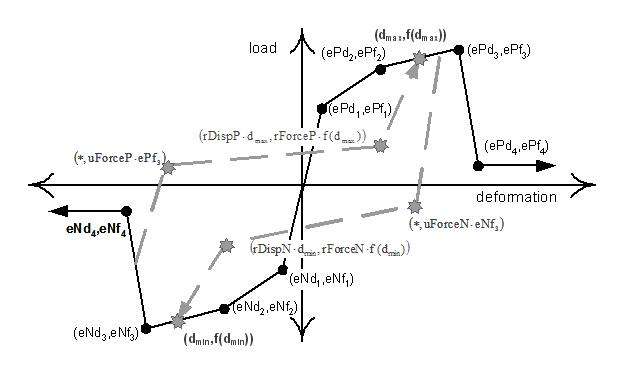
\includegraphics[width=9cm]{figures/Pinching4.jpg}
  \caption{Representation of the capacity curve required to represent the structural capacity of the SDoF system.}
  \label{fig:backbone}
\end{figure}

It can be noted that the capacity curve can describe only the envelope response of the hysteretic behaviour. In order to keep the definition of the model as simple as possible, some assumptions have been formulated on the unload-reload path and the three damage rules.\\

The first assumption regards the level of pinching of the cyclic behaviour. rDispP, rForceP and uForceP (see Figure \ref{fig:backbone}) are the parameters that control the unload-reload paths of Pinching4 material; they are assigned default values of 0.5, 0.25 and 0.05, respectively to represent a medium level of pinching. Since the cyclic behaviour is considered symmetrical the parameters rDispN, rForceN and uForceN are set equal to rDispP, rForceP and uForceP, respectively.
The second assumption regards the degrading behaviour of the model. The user has the option of introducing energy-based degradation during the cyclic hystory assigning non-zero values to the parameters gK2, gD2 and gF2, that control unloading, reloading stiffness and strength degradation, respectively. If degradation is selected gK2, gD2 and gF2 are assigned default values of 0.1, 0.1 and 0.4 respectively. More details about the degrading models and the meaning of the degrading parameters can be found in \citep{LowesEtAl2003}  and in the OpenSees wiki (\href{http://opensees.berkeley.edu/wiki/index.php/Pinching4_Material}{http://opensees.berkeley.edu/wiki/index.php/Pinching4\_Material}).\\

If the User agrees with these assumptions he should set the variable \verb=sdof_hysteresis= to \verb="Default"= in the ipython notebook

\begin{Verbatim}[frame=single, commandchars=\\\{\}, samepage=true]
sdof_hysteresis = "Default"
\end{Verbatim}

If the User wants instead to define each variable of the pinching4 material himself, he should assign the variable \verb=sdof_hysteresis= the path to the file where these parameters are specified.

\begin{Verbatim}[frame=single, commandchars=\\\{\}, samepage=true]
sdof_hysteresis = "../../../../../rmtk_data/pinching_parameters.csv"
\end{Verbatim}

The pinching parameters should be defined in a csv file (tabular format) as shown in Table \ref{table:pinching4}. The variables of Table \ref{table:pinching4} are those characterising pinching4 material as explained in the OpenSees wiki (\href{http://opensees.berkeley.edu/wiki/index.php/Pinching4_Material}{http://opensees.berkeley.edu/wiki/index.php/Pinching4\_Material}).

\begin {table}[htb]
\caption{Example of file containing Pinching4 material parameters}
\label{table:pinching4}
\begin{center}
  \begin{tabular}{ | c | c | c | c | c | c |}
  \hline
	rDisp  & 0.4	&	&	&	 &	\\ \hline
	fForce	 & 0.6 &	&	&	 &	\\ \hline
	uForce	 & 0	&	&	&	 &	\\ \hline
	gK1	 & 0  &	0.6  &	0  &	0	 & 1\\ \hline
	gD1	 & 0	 & 0  &	0  &	0  &	0\\ \hline
	gF1	 & 0  &	0.07	 & 0  &	0.07  &	0.9\\ \hline
	gE	 & 10 &	&	&	 &\\ \hline
	dmgType	& energy &	&	&	 &\\ \hline
	\end{tabular}
\end{center}
\end{table}			

In order to use this methodology, it is necessary to load one or multiple capacity curves and a set of ground motion records, as explained in Sections~\ref{subsec:cap_curves} and \ref{subsec:gmrs}, respectively. Then, it is necessary to specify a damage model using the parameter \verb=damage_model=. 
Currently spectral displacement, capacity curve-based and inter-storey drift-based damage criterion can be used in the damage model (see Section~\ref{subsec:dmg_model}). When the capacity curve-based criterion is selected, it may be necessary to identify the yielding spectral displacement and acceleration. The User can either input the yielding point in the input file, or he can use the algorithm described in Section \ref{subsec:cap_curves} for the idealisation of the capacity curves, to identify the spectral displacement and acceleration at yielding on the capacity curves. When inter-storey drift-based damage criterion is selected it is necessary to define a file containing the relationship between maximum inter-storey drift and spectral displacement (see Section~\ref{subsubsec:isd_dmg}). If this file is not defined a linear relationship between inter-storey drift and roof displacement is assumed and the spectral displacement is obtained dividing the roof displacement by the first modal participation factor $\Gamma$. \\

The damping ratio must be defined using the parameter \verb=damping=, and if structural degradation should be considered in the analysis, it is necessary to set the parameter \verb=degradation= to \verb=True=. After importing the module \verb=NLTHA_on_SDOF=, it is possible to calculate the distribution of structures across the set of damage states for each ground motion record using the following command:

\begin{Verbatim}[frame=single, commandchars=\\\{\}, samepage=true]
PDM, Sds = NLTHA_on_SDOF.calculate_fragility(capacity_curves,gmrs,...
damage_model,damping)
\end{Verbatim}

Where \verb=PDM= (i.e. probability damage matrix) represents a matrix with the number of structures in each damage state per ground motion record, and \verb=Sds= (i.e. spectral displacements) represents a matrix with the maximum displacement (of the equivalent SDoF) of each structure per ground motion record. The variable PDM can then be used to calculate the mean fragility model as described in Section \ref{subsec:derive_fragility}.